%********************************************
\chapter{Related Work}\label{ch:related-work}
%********************************************

As information disorder continues to evolve, so too do surveys of research efforts in combatting it constantly diversify. This is markedly the case for scientific approaches. This diversity in perspectives and approaches indicates the complexity of information disorder. It also signifies the necessity for a holistic view of the problem.

\section{Misinformation detection with Machine Learning}
\label{sec:2-mdml}

Existing approaches to misinformation detection using news text data generally involve two subtasks: feature extraction, and learning and classification.

\subsection{Feature extraction}
\label{ssec:2-feature-extraction}

Feature extraction is a process by which attributes of news items on \ac{OSN} posts are extracted and processed for classification. \citeauthoryear{Shu:2017} categorised these features into two groups, based on: (i.) news content, \emph{i.e.}, text and image features; and (ii.) social context, \emph{i.e.}, features based on users, posts, and networks.

Numerous papers use text features to detect fake news. Being the feature of interest in this work, this is expanded on in \sectionref{sec:2-existing} and \sectionref{sec:2-text}. In addition to images, videos and speeches are also used to extract features for fake news detection. Multiple features can be combined for detection, \emph{i.e.}, in a \emph{multimodal} fashion. \citeauthoryear{Alam:2022} surveyed multimodal fake news detection. Similarly, \citeauthoryear{Cao:2020} gave a comprehensive overview of the role visual content plays in fake news detection, while \citeauthoryear{Shu:2020b} did the same for user profiles. \citeauthoryear{Zhou:2019}, and \citeauthoryear{Shu:2020c} demonstrate the application and efficacy of network-based features.


\subsection{Learning and classification}
\label{ssec:2-learning-and-classification}

An \ac{ML} model is then trained using the extracted features, to classify new, unseen news items or posts. The training process can be:
\begin{itemize}
  \item \underline{Supervised}: data with labels (typically `real' or `fake') are applied to train a classifier, \emph{e.g.} neural network, decision tree, \ac{SVM}, \emph{etc.}
  \item \underline{Semi-Supervised}: this approach primarily aims to attenuate reliance on labelled data, which may be insufficient. It leverages unlabelled data to make predictions with higher accuracy than would have been attained using only labelled data.\sidecite{Ouali:2020} Commonly known examples include:\sidenote{Ibid.}
  \begin{itemize}
    \item generative models, which initially learn features from a given task and are afterwards used in other tasks.
    \item proxy-label methods, which utilise a model trained on a labelled dataset to generate more training data by labelling examples of unlabelled data.
    \item graph-based methods, which model labelled and unlabelled data as nodes in a graph and try to propagate labels from the former to the latter.
  \end{itemize}
  Semi-supervised learning also allows for a human-in-the-loop detection process. Some of the data are unlabelled in this case. An example is \emph{active learning}, whereby labels for the most ambiguous training examples are sought from a human—a content moderator, for instance—to progressively improve the classification accuracy.
  \item \underline{Unsupervised}: all data are unlabelled in this case. The task could be one of clustering, or anomaly detection whereby a fake news item is picked up as an outlier in the dataset.
\end{itemize}

Though wanting in visualisation, the overview of information disorder given by \citeauthoryear{Zannettou:2019}, which is based on the work of \citeauthoryear{Wardle:2017},\sidenote{See \sectionref{sec:1-infodis}.} is sufficiently encompassing. It includes the various types of false information, its actors, as well as their motivations. Furthermore, works that analyse how false information propagates via different \acp{OSN}, as well as those which focus on how to detect them, are discussed. By comparison, \citeauthoryear{Wardle:2017b} equally gives a comprehensive view of the ecosystem—additionally, with a visual illustration to better the reader’s understanding—of the types, actors, motives and phases of misinformation. However, a similar illustration for existing computational approaches is lacking in the literature.

\autoref{fig:taxonomy} shows a taxonomy of the different methods used to detect fake news and the sub-classification of tasks within each. In the following subsection, examples from the literature of each method and features utilised will be discussed.

\renewcommand{\imsize}{\linewidth}%
\begin{figure}[htb]%
	\noindent\makebox[\textwidth]{%
		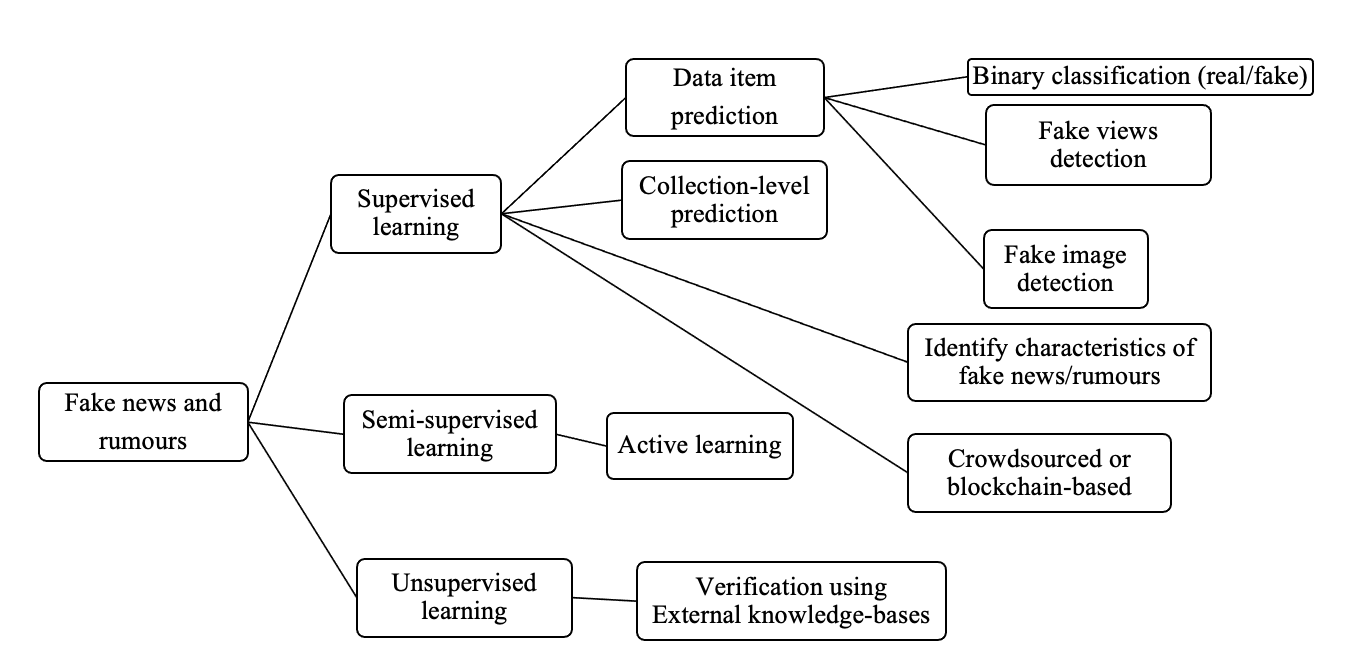
\includegraphics[width=\imsize]{gfx/taxonomy}%
	}%
	\caption[Fake news detection taxonomy]{Fake news detection taxonomy.}%
	\label{fig:taxonomy}%
\end{figure}%

\section{Text representations for misinformation detection}
\label{sec:2-existing}

Although today it is produced and consumed in various media, news has pre-eminently been circulated in textual form. Over time, textual news developed into a general ossified structure:

\begin{itemize}
    \item Source: the author and/or publisher of the article.
    \item Headline/title: this typically is a short sentence, descriptive of the principal news topic covered in the article.
    \item Body: the main text of the article, detailing the news story.
    \item Image/video: visual (or audio-visual) cue(s) included in the body of the article.
\end{itemize}

\newthought{In an in-depth} study of the structure of news, \citeauthoryear{Dijk:1983} described the news as having two kinds of structure: thematic and schematic. The former represents the topical contents of a news item, while the latter describes the structure of the item's discourse. In other words, a news item is composed of themes bound together by a schema. These themes may vary (in nature and style of presentation) from one article to another, but the schema is firmly established.\sidenote{\citeauthor{Dijk:1983}'s study and conclusions were based on an empirical study of global press coverage of the 1982 assassination of the Lebanese president-elect, Bachir Gemayel. It covers 700 news articles published by 250 newspapers from 100 countries.}

Online news presumably inherits its structure from that of traditional, printed news. Though the visual layout may be notably different. For instance, news on the web is typically laid out in a single, rather than multiple columns, has `share' buttons, \emph{etc.} However, its schema is identical to that of print news. Implicit in this schema, is a top-to-bottom outline of the news content, ranked from the most to the least important or newsworthy fragments.\sidecite{Dijk:1983} It is conventional for journalists to produce—as it is for readers to assimilate—news in this manner. It is likely, therefore, for the most relevant textual content for news analysis to be found closer to the top, rather than at the bottom of the news item.

Although published nearly four decades ago—long before the dawn of news detection using \ac{NLP} and \ac{ML}—\citeauthor{Dijk:1983}'s paper provides some interesting and practical insights that could inform its current modus operandi. For instance, he gleaned from his study, that:

\begin{itemize}
    \item the paramount topic of a news item is captured in its headline; and
    \item the opening sentences and paragraphs form the top of the schema—containing crucial details such as the time, location, parties, causes and outcomes of the main news events.
\end{itemize}

To summarise, the hierarchical structure of news embodies a linearly decreasing ordering of thematic information in a news item, from top to bottom. van Dijk attributes this order to ``an implicit journalistic rule of the news organization.'' As news is written, so it is read. Thus, one can catch the scope of a news item by simply reading the headline and the main details in the opening section. This is true for most authentically produced news articles that adhere to journalistic standards. However, news produced with bad intent can exploit the hierarchy of its content for mal-intent.

Some have attempted to take advantage of this hierarchy for misinformation detection,\sidenote{For example, \citeauthoryear{Biyani:2016} used features, including titles, extracted from news webpages to detect clickbait; \citeauthoryear{Sisodia:2019} extracted features from headlines to do the same; while \citeauthoryear{Yoon:2019} assessed the congruity between news headlines and body texts.} while most works using text data have relied on the body of articles. One of the main contributions of this thesis is that it presents a way to harness the inherent schematic of news, for detecting misinformation.


\section{Use of text in ML-based misinformation detection research}
\label{sec:2-text}

Whereas photos and videos were once merely accompaniments to news pieces, they are gradually taking centre stage in news dissemination, especially on \acp{OSN}. Nonetheless, text remains the predominant and most abundant form of news. Similarly, misinformation proliferating through social media and the web is typically in the form of text, and photos or videos are only recent developments. Besides, text can be extracted from news items disseminated in pictorial or video forms for analysis. For example, text extracted from a news video through speech-to-text technology can be used for \ac{NLP} analysis. Text can similarly be extracted from photos. Expectedly, research in misinformation detection has mostly utilised text data as raw material, and \ac{NLP} and \ac{ML} techniques for extraction, enrichment and categorisation.

This research explores text representations for detecting online misinformation. In other words, it aims to find effective means of transforming text data into meaningful representations that can be used to characterize or identify fake news.

This section describes an overview of some key papers on text representations for misinformation detection. Most papers selected for this discussion focus their approach on two main strategies for exploiting textual data:

\begin{enumerate}
    \item text-based features, generally extracted from the body text.
    \item the schema of news: \emph{i.e.}, papers which exploit features from a specific portion of news articles, such as headlines.
\end{enumerate}

This section will focus on text-based features used for misinformation detection using \ac{ML}. \citeauthoryear{Shu:2019b} categorises such features into three groups: (i.) linguistic, (ii.) low-rank,  and (iii.) neural text features. More elaborately, \citeauthoryear{Zhou:2020} additionally categorise linguistic features into four groups: (i.) lexical, (ii.) syntactic, (iii.) discourse, and (iv.) semantic.

\newthought{Linguistic features aim} to capture the \emph{style} of writing in a piece of text. From this style, intent may be inferred (\emph{i.e.}, whether to mislead or not),\sidecite{Zhou:2020} or characterisation can be made (since fake news will likely have a style that differs from that of authentic news).

The following are some linguistic features and their applications for fake news detection:\sidenote{\citeauthoryear{Shu:2019b}, \citeauthoryear{Zhou:2020}}

\begin{itemize}
    \item Lexical features are generally concerned with the tallies or frequencies of character- or word-level features. Examples include $n$-grams, \ac{BoW} methods, and \ac{TFIDF}, which captures the relevance of a given word to a document in a corpus. Another is the \ac{LIWC}, which calculates what percentage of words in a text fall into one of many categories, which indicate emotional and psychological properties, amongst others.

    \item Syntactic features are typically sentence-level features, including counts of punctuations, words, phrases, \ac{PoS} tagging, and \ac{PCFG} parse trees. Additional examples of these features are those specific to the news domain, such as quotations and links.

    \item Discourse features include applications of the \ac{RST} and rhetorical parsers to extract rhetorical features from sentences.

    \item Latent features are primarily embeddings created using deep neural networks such as \acp{CNN}, \acp{RNN} (particularly, using the \ac{LSTM} architecture), and Transformers. These embeddings are dense vector representations of text at the word (most commonly), sentence, or document level. Commonly used word embedding models include \texttt{word2vec}\sidecite{Mikolov:2013}, and more recently, transformer-based architectures such as BERT\sidecite{Devlin:2019} and its variants. Another latent feature that is particularly relevant to this work (in \autoref{ch:thematic-coherence}) is the topic feature, extracted using topic modelling. Topic models identify themes latent in a group of documents by analysing the distribution of words and/or phrases across them.\sidecite{Blei:2012}
\end{itemize}


\citeauthoryear{Casillo:2021} used a} combination of topics, syntactic, and semantic features from news texts in three datasets to detect misinformation. They obtained the topic features using the \ac{LDA} topic model. \ac{LDA} is also used in this work and an in-depth explanation of its workings is given in \sectionref{ssec:4-LDA}. Stopwords were removed before feature extraction.\sidenote{stopwords are words such as \emph{`just'}, \emph{`do'}, and \emph{`it'}, which are non-descriptive, and therefore, relatively less insightful with regard to generating or interpreting topics.} They used three syntactic features: (i.) the number of characters; (ii.) the Flesch Index, which is a measure of text readability; and (iii.) the Gunning Fog Index, which estimates text comprehensibility. These features are further processed using the \ac{CDT}, which aids the selection of topics using temporal context. Next, they incorporate two semantic features—the probabilities of negative and positive news sentiment. Finally, the features are fed into a \ac{kNN} classifier for detection.

Another work that uses topic features is by \citeauthoryear{Hosseini:2022}. Similar to the previous work, an \ac{LDA} topic model was used to extract features. Before this, though, the texts are preprocessed into tokens, and non-English words and stopwords are removed. Word embeddings are obtained from the original news texts using the \texttt{word2vec} model. These embeddings are input into a bi-directional \ac{LSTM} \ac{VAE} to form latent representations of the texts. The \ac{VAE} representations are combined with the \ac{LDA} topic representations to form the final features for classification. The combined features improved misinformation detection for classifiers compared to individual features.

Topic features can be extracted from non-English news texts. They can also be used for tasks other than detection. For example, \citeauthoryear{Paixao:2020} used \ac{BoW}, word embedding, \ac{LIWC}, \ac{PoS}, and \ac{TFIDF} features to differentiate between real and fake news in a Brazilian Portuguese news corpus. However, they further employed topic modelling to qualitatively study the two groups of articles in the dataset. They found the optimal number of topics to analyse using the coherence measure. This is also used in this work, although in a different way, in \sectionref{ssec:4-coherence-perplexity}.

\ac{LDA} is not the only topic modelling method available, but it is more commonly used in the literature. \citeauthoryear{Ajao:2019} experimented with a different method called \ac{LSA}, but found \ac{LDA} to perform better. They applied topic modelling to determine the 10 most prevalent topics in rumour and non-rumour tweets. The sentiment (positive, negative, or neutral) values of the words in each topic were then computed and used to calculate an \emph{emotional ratio score}. This score was combined with linguistic features such as counts of user mentions, hashtags, and quotations, to form features for rumour detection.

\autoref{tab:mlformisinfo} shows some of the commonly used text-based features for misinformation detection and examples of papers wherein they are implemented.

\begin{threeparttable}
\addlinespace
\begin{tabularx}{\linewidth}{>{\raggedright}p{2cm}X}
  \toprule

  \tableheadline{\shortstack[l]{Text Feature}} &
  \tableheadline{\shortstack[l]{Papers Implemented In}}  \\
  \midrule

  Lexical &
  \ac{BoW}: \citeauthoryear{Paixao:2020}, \citeauthoryear{Zhou:2020b}; \newline
  \ac{LIWC}: \citeauthoryear{Perez-Rosas:2018}, \citeauthoryear{Paixao:2020}; \newline
  $n$-grams: \citeauthoryear{Biyani:2016}, \citeauthoryear{Ahmed:2017}, \citeauthoryear{Potthast:2018}; \newline
  \ac{TFIDF}: \citeauthoryear{Biyani:2016}; \citeauthoryear{Perez-Rosas:2018} \newline
  Others: \citeauthoryear{Biyani:2016}, \citeauthoryear{Potthast:2018}, \citeauthoryear{Yang:2019}, \citeauthoryear{Paixao:2020} \\
  \midrule

  Syntactic &
  \ac{PoS}: \citeauthoryear{Feng:2012}, \citeauthoryear{Potthast:2018}, \citeauthoryear{Paixao:2020}, \citeauthoryear{Zhou:2020b}; \newline
  \ac{PCFG}: \citeauthoryear{Feng:2012}, \citeauthoryear{Perez-Rosas:2018}, \citeauthoryear{Zhou:2020b}; \newline
  Others: \citeauthoryear{Potthast:2018} \\
  \midrule

  Discourse &
  \ac{RST}: \citeauthoryear{Rubin:2015}; \newline
  Others: \citeauthoryear{Karimi:2019}, \citeauthoryear{Zhou:2020b} \\
  \midrule

  Latent &
  \ac{CNN}: \citeauthoryear{Wang:2017b}, \citeauthoryear{Ajao:2018}, \citeauthoryear{Yang:2018}; \newline
  \ac{RNN}: \citeauthoryear{Rashkin:2017}, \citeauthoryear{Ruchansky:2017}, \citeauthoryear{Ajao:2018}, \citeauthoryear{Karimi:2019}, \citeauthoryear{Zhang:2019}, \citeauthoryear{Hosseini:2022}; \newline
  Transformers: \citeauthoryear{Vijjali:2020}, \citeauthoryear{Kula:2021}, \citeauthoryear{Raza:2022} \newline
	Topics: \citeauthoryear{Bhattacharjee:2018}, \citeauthoryear{Ajao:2019}, \citeauthoryear{Benamira:2019}, \citeauthoryear{Li:2019} \\
  \bottomrule

\end{tabularx}
\caption{Some of the main text representations for misinformation detection}
\label{tab:textrepsformisinfo}
\end{threeparttable}
\newline\bigskip

\newthought{Similar to \citeauthoryear{Zannettou:2019},} \citeauthoryear{Zubiaga:2018} provide a comprehensive overview of research in this field, specifically focusing on rumours on \acp{OSN}. They categorise rumour classification architectures into four main types: \emph{rumour detection}, \emph{rumour tracking}, \emph{stance classification}, and \emph{veracity classification}. Additionally, they discuss examples of scientific approaches taken and datasets used by researchers to tackle each task—along with the state-of-the-art method for each task.

This research is primarily concerned with misinformation detection using machine learning. The availability of data is a prerequisite to achieving this goal. Furthermore, there are different \ac{ML} approaches that can and have been used to solve this problem. In this section, existing datasets and \ac{ML} approaches for misinformation detection are reviewed.

This thesis extends \citeauthoryear{Zubiaga:2018} by further categorising the \ac{ML} approaches cited in it—and incorporating those cited in other papers supervised, semi-supervised and unsupervised, as is laid out in \autoref{tab:mlformisinfo}. It also expands on the applicable datasets for the respective tasks cited in \citeauthoryear{Zubiaga:2018}. Their work focuses on rumours, while this research targets the broader ecosystem of misinformation. Note that the information in \autoref{tab:mlformisinfo} does not constitute an exhaustive list of published research papers or datasets in each category.

\begin{threeparttable}
\addlinespace
\begin{tabularx}{480pt}{>{\raggedright}p{2cm}>{\raggedright}p{3cm}>{\raggedright}p{3cm}>{\raggedright}p{3cm}X}
  \toprule

  \tableheadline{\shortstack[l]{ML \smallskip\\ Approach}} &
  \tableheadline{\shortstack[l]{Misinformation \smallskip\\ Detection}} & \tableheadline{\shortstack[l]{Misinformation \smallskip\\ Tracking}} &
  \tableheadline{\shortstack[l]{Stance \smallskip\\ Classification}} &
  \tableheadline{\shortstack[l]{Veracity \smallskip\\ Classification}}  \\
  \midrule

  Supervised & \citeauthoryear{Wu:2015}, \citeauthoryear{Zubiaga:2016}, \citeauthoryear{Ahmed:2017}, \citeauthoryear{Ruchansky:2017}, \citeauthoryear{Wang:2018}, \citeauthoryear{Wu:2018}, \citeauthoryear{Zhang:2020} &

  \citeauthoryear{Castillo:2011}, \citeauthoryear{Ruchansky:2017}, \citeauthoryear{Wang:2017} &

  \citeauthoryear{Kochkina:2017}, \citeauthoryear{Shang:2018} &

  \citeauthoryear{Castillo:2011}, \citeauthoryear{Kwon:2017} \\

  \midrule

  Semi-supervised & \citeauthoryear{Bhattacharjee:2018}, \citeauthoryear{Guacho:2018}, \citeauthoryear{Shu:2019} & — & — & — \\
  \midrule

  Unsupervised & \citeauthoryear{Chen:2016}, \citeauthoryear{Zhang:2016}, \citeauthoryear{Zhang:2017}, \citeauthoryear{Chen:2018}, \citeauthoryear{Hosseinimotlagh:2018} & — & — & — \\
  \bottomrule

  \spacedlowsmallcaps{Dataset} &
  \citeauthoryear{Mitra:2015}, \citeauthoryear{Zubiaga:2016}, \citeauthoryear{Zubiaga:2016b}, \citeauthoryear{Zubiaga:2016c}, \citeauthoryear{Kwon:2017}, \citeauthoryear{Kochkina:2018}, \citeauthoryear{Shu:2018}, \citeauthoryear{Rubin:2019} &
  \citeauthoryear{Kochkina:2018} &
    \citeauthoryear{Zubiaga:2016c}, \citeauthoryear{Mohammad:2016}, \citeauthoryear{Mohammad:2017}, \citeauthoryear{Kochkina:2018}, \citeauthoryear{Gorrell:2019} &
  \citeauthoryear{Zubiaga:2016c}, \citeauthoryear{Kwon:2017}, \citeauthoryear{Kochkina:2018}, \citeauthoryear{Gorrell:2019}, \citeauthoryear{Rubin:2019}, \citeauthoryear{Arslan:2020} \\
  \bottomrule
\end{tabularx}
\caption{A breakdown of existing \ac{ML} architectures for misinformation classification.}
\label{tab:mlformisinfo}
\end{threeparttable}

\newthought{The literature on} misinformation detection has been mostly focused on supervised learning. \citeauthoryear{Castillo:2011} were among the earliest to evaluate the veracity of \ac{OSN} content using supervised learning. Their objective was to assess how believable tweets about global news events were over two months. They generated a dataset of 747 tweets, manually labelled (`true' or `false') by expert judges. Extracted features were topic-based (\emph{e.g.} textual length and sentiment of tweet), network-based (\emph{e.g.} the number of users’ followers), propagation-based (\emph{e.g.} total number of tweets) and top-element (\emph{e.g.} fraction of tweets containing the most popular hashtag). They tried four different supervised \ac{ML} methods including \acp{SVM} and Bayes networks, but Decision Trees yielded the highest accuracy.

\citeauthoryear{Ruchansky:2017} created a deep learning model to detect fake news, using Twitter and Weibo data. It consists of three modules: \emph{Capture}, \emph{Score} and \emph{Integrate}. The Capture module is built using a \ac{RNN} which represents the temporal dynamics of a user’s activities, and a \texttt{doc2vec} representation\sidecite{Mikolov:2014} of text posted therein. In the Score module, a neural network assigns a score to a user, based on their tendency of being the source of a fake news article. The third module combines information from the first two to classify the article. Supervised \ac{ML} has also been used to detect rumours by analysing how they propagate. \citeauthoryear{Wu:2015} achieved this using an \ac{SVM} classifier, while \citeauthoryear{Wu:2018} used \acp{RNN}.

\newthought{Given that in} real-world scenarios, labelled data is—at least immediately—lacking, some have tried to eliminate this restraint. \citeauthoryear{Shu:2019} proposed a novel semi-supervised approach, which models the interrelationship between the contents, publishers, and users (consumers) of news items (of which some are labelled). It predicts the unlabelled news items, using features extracted from the news articles, social relations between users, users' engagements with the news articles, and publishers’ partisan associations. They collated fact-check data from BuzzFeed\sidenote{\raggedright\url{https://github.com/BuzzFeedNews/2016-10-facebook-fact-check/tree/master/data}}, PolitiFact\sidenote{\raggedright\url{https://www.politifact.com/factchecks}} and Media Bias/Fact-Check\sidenote{\raggedright\url{https://mediabiasfactcheck.com}}, into two new datasets\sidecite{Shu:2018}, which both included information on news contents, publishers and social interactions. They simplified the embeddings of their features using \ac{NMF} and devised an optimisation algorithm to classify the news articles.

\citeauthoryear{Bhattacharjee:2018} used active learning to detect the veracity of news, using partially labelled datasets. Their system comprises two simultaneously running, independent modules. The first module $M_1$ begins with a Logistic Regression classifier and a copy of the labelled dataset. It selects and assigns weights to features by iteratively computing the Joint Mutual Information Maximisation between features and class labels, and gives higher weights to the most relevant ones in a greedy way. $M_1$’s dataset is updated to include the assigned weights, and the classifier is retrained. The second module $M_2$ begins with a copy of the unlabelled and labelled dataset. The latter was used to train an underlying classification model which is based on a \ac{CNN}. Both modules iteratively classify each unlabelled sample, and they request labels from a human if their predictions do not attain a preset certainty threshold. $M_1$ and $M_2$ update their training sets to include the given labels, and then fine-tune their classification models. Finally, the predictions from both modules are combined into a decision profile and a fusion classifier was used to make a final decision on a sample.

The advantage of unsupervised learning is neither labelled data nor human input is needed. \citeauthoryear{Zhang:2016} considered fake news detection as an outlier detection problem. The rationale behind this is that the behaviours (related to style and timing) of a user when posting rumours and non-rumours will differ. Thus, rumours can be picked up as outliers in the user’s feed. They used \ac{PCA} to detect rumours on Weibo. They initially collected verified rumour and non-rumour posts for analysis, to determine relevant features. The 13 selected features were numerical and categorical. When a post is flagged as a rumour, their model collects a set of $N$ recent posts (between 10 and 100) by the poster and extracts the aforesaid features from them.
The model then performs \ac{PCA} which transforms the $N$ posts into a matrix with $N$ rows (posts, the first of which denotes the original flagged post) and eight columns containing quantitative values. Eight was analytically chosen as the optimal number of primary components as it is the smallest number which captured at least 85\% of the total variance in the recent posts, using varying $N$ sample sizes. The original post is considered an outlier (\emph{i.e.}, a rumour) if it does not have at least zero neighbours within a given distance: calculated as the mean distance between pairs of posts divided by the standard deviation.


\section{Limitations of existing methods}
\label{sec:2-limitations}

Given the significance of information disorder, a lot of work has been done to address many of its subproblems. However, some limitations remain unsolved. The following are some limitations related to this thesis:

\begin{enumerate}
    \item One of the open challenges in contemporary fake news research is the lack of cross-domain, cross-topic, and cross-language studies.\sidenote{\citeauthoryear{Zafarani:2019}, \citeauthoryear{Zhou:2020}} This thesis partly addresses this limitation through the use of cross-domain datasets, that cover several different news topics, for fake news detection.

    \item Although extensively used to engineer features for fake news detection,\sidenote{See \sectionref{sec:2-text}.} stylometric features are ineffective for distinguishing between genuine news and fake news autogenerated by language models.\sidecite{Schuster:2020} This limitation may be overcome by exploring features which transcend stylometry, such as topics, which are used in this work.

    \item Large amounts of labelled data are needed to create accurate models, as observed by \citeauthoryear{Wu:2018} and \citeauthoryear{Wang:2017b}. This is a motivation for using unsupervised \ac{ML}, in which case a labelled dataset is not a prerequisite. The process of manually annotating datasets can be costly and very time-consuming. Furthermore, while some authors have employed Amazon Mechanical Turk workers to annotate their datasets, others\sidenote{\citeauthoryear{Castillo:2011}, \citeauthoryear{Mitra:2015}, \citeauthoryear{Vosoughi:2018}, \citeauthoryear{Zhang:2018}} preferred to use trained annotators, claiming that they made more informed judgements on the veracity of examples. This ascribes an element of doubt to the reliability of manually labelled datasets.
\end{enumerate}
